\chapter[Alocação de Tarefas em Sistemas Multi-Robôs]{Alocação de Tarefas em Sistemas Multi-Robôs} \label{cap:mrta}

    Um dos problemas mais desafiadores em aplicações multi-robôs é denominado como \textit{alocação de tarefas}, (MRTA, acrônimo para \textit{Multi-Robot Task Allocation}). Problemas dessa natureza buscam como solução atribuir otimamente um conjunto de robôs para um conjunto de tarefas de maneira que o desempenho geral de um sistema sujeito a um conjunto de limitações seja otimizado.
    
    \textcolor{red}{falar sobre o conteúdo deste capítulo}
    
    \section{Definição Formal} \label{sec:sec3_1}
        Colocar texto aqui
    
    \section{Taxonomias} \label{sec:taxonomias}
        
        \citeonline{ref:gerkey2004taxonomy} sugeriram uma taxonomia de três eixos independente do domínio de para a classificação de problemas de alocação de tarefas em sistemas multi-robôs. 
        
        O primeiro eixo determina o \textit{tipo dos robôs} que compõem o problema. Os tipos de robôs possíveis são: \textit{ST} (acrônimo para \textit{Single-Task}) ou \textit{MT} (acrônimo para \textit{Multi-Task}). Problemas que envolvem robôs que só podem executar uma tarefa por vez são compostos por robôs do tipo \textit{ST}. Entretanto, se houver pelo menos um robô capaz de executar mais de uma tarefa simultaneamente, então esse problema é composto por robôs do tipo \textit{MT}. 
        
        O segundo eixo da taxonomia determina o \textit{tipo das tarefas} que compõem o problema. Nesse caso, são possíveis os tipos: \textit{ST} (acrônimo para \textit{Single-Robot}) ou \textit{MR} (acrônimo para \textit{Multi-Robot}). Problemas cujo tipo das tarefas é \textit{SR}, diz-se que todas as tarefas envolvidas só podem ser executadas por um robô. Porém, quando o tipo das tarefas envolvidas é \textit{MR}, diz-se que existe tarefas que podem ser executadas por mais de um robô.
        
        O terceiro eixo, por sua vez, determina o \textit{tipo da alocação} do problema, o qual pode assumir os valores: \textit{IA} (acrônimo para \textit{Instantaneous Assignment}) ou \textit{TA} (acrônimo para \textit{Time-extended Assignment}). O primeiro caso, \textit{IA}, diz repeito à problemas MRTA onde as alocações das tarefas para os robôs são realizadas instantaneamente, sem levar em consideração o estado futuro do sistema. Por outro lado, em problemas cujo tipo de alocação é \textit{TA}, além de conhecido o estado atual de cada rôbo e do ambiente, também é conhecido o conjunto de tarefas que precisarão ser alocadas no futuro. Neste último caso, diversas tarefas são alocadas para um robô, o qual deve executar cada alocação conforme seu agendamento. De acordo com \cite{ref:bastos2008utility}, quando o tipo de alocação do problema MRTA é \textit{IA}, o número de robôs é superior ao número de tarefas alocadas e quando \textit{TA}, o oposto acontece. Isso se deve ao fato de que, em problemas MRTA cujo tipo de alocação é \textit{IA}, o número de robôs no sistema é capaz de suprir a taxa de tarefas a serem atribuídas, de modo que é muito provável que haverão robôs ociosos no sistema; enquanto, naqueles cujo tipo de alocação é \textit{TA}, o número de robôs que compõem o sistema não é suficiente para atender a taxa de tarefas a serem alocadas no sistema.
        
        \begin{figure}[htb]
            \centering
            % Graphic for TeX using PGF
% Title: ../figures/taxonomia_mrta.dia
% Creator: Dia v0.97.2
% CreationDate: Tue Oct 17 17:33:09 2017
% For: adrianohrl
% \usepackage{tikz}
% The following commands are not supported in PSTricks at present
% We define them conditionally, so when they are implemented,
% this pgf file will use them.
\ifx\du\undefined
  \newlength{\du}
\fi
\setlength{\du}{15\unitlength}
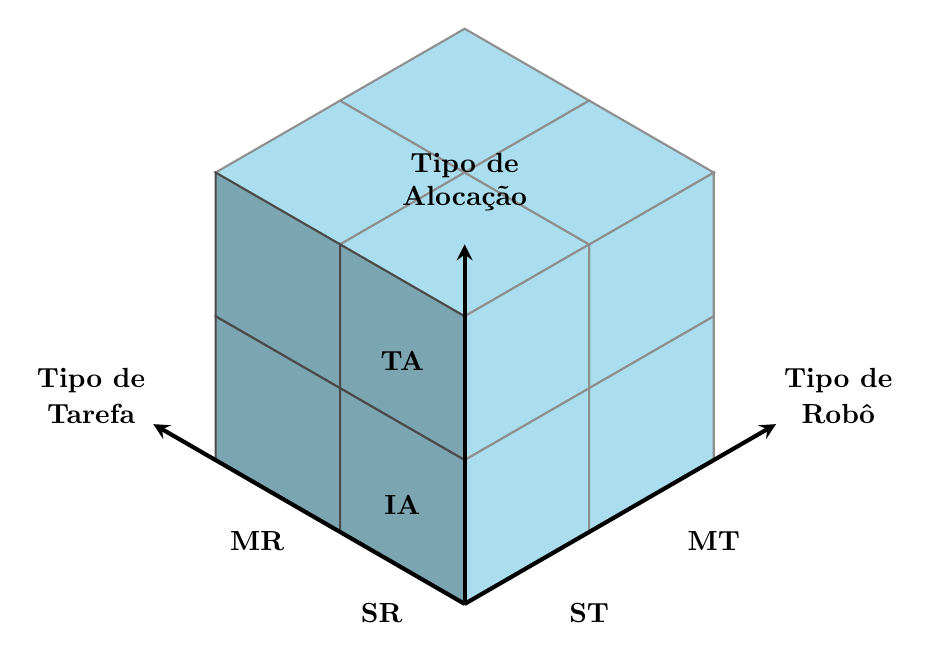
\begin{tikzpicture}
\pgftransformxscale{1.000000}
\pgftransformyscale{-1.000000}
\definecolor{dialinecolor}{rgb}{0.000000, 0.000000, 0.000000}
\pgfsetstrokecolor{dialinecolor}
\definecolor{dialinecolor}{rgb}{1.000000, 1.000000, 1.000000}
\pgfsetfillcolor{dialinecolor}
\pgfsetlinewidth{0.050000\du}
\pgfsetdash{}{0pt}
\pgfsetdash{}{0pt}
\pgfsetmiterjoin
\pgfsetbuttcap
\definecolor{dialinecolor}{rgb}{0.666667, 0.870588, 0.937255}
\pgfsetfillcolor{dialinecolor}
\fill (-5.500000\du,-10.392300\du)--(-2.500000\du,-8.660250\du)--(0.500000\du,-10.392300\du)--(-2.500000\du,-12.124400\du)--cycle;
\definecolor{dialinecolor}{rgb}{0.556863, 0.556863, 0.556863}
\pgfsetstrokecolor{dialinecolor}
\draw (-5.500000\du,-10.392300\du)--(-2.500000\du,-8.660250\du)--(0.500000\du,-10.392300\du)--(-2.500000\du,-12.124400\du)--cycle;
\pgfsetlinewidth{0.050000\du}
\pgfsetdash{}{0pt}
\pgfsetdash{}{0pt}
\pgfsetmiterjoin
\pgfsetbuttcap
\definecolor{dialinecolor}{rgb}{0.666667, 0.870588, 0.937255}
\pgfsetfillcolor{dialinecolor}
\fill (-2.500000\du,-12.124400\du)--(0.500000\du,-10.392300\du)--(3.500000\du,-12.124400\du)--(0.500000\du,-13.856400\du)--cycle;
\definecolor{dialinecolor}{rgb}{0.556863, 0.556863, 0.556863}
\pgfsetstrokecolor{dialinecolor}
\draw (-2.500000\du,-12.124400\du)--(0.500000\du,-10.392300\du)--(3.500000\du,-12.124400\du)--(0.500000\du,-13.856400\du)--cycle;
\pgfsetlinewidth{0.050000\du}
\pgfsetdash{}{0pt}
\pgfsetdash{}{0pt}
\pgfsetmiterjoin
\pgfsetbuttcap
\definecolor{dialinecolor}{rgb}{0.666667, 0.870588, 0.937255}
\pgfsetfillcolor{dialinecolor}
\fill (3.500000\du,-8.660250\du)--(3.500000\du,-5.196150\du)--(6.500000\du,-6.928200\du)--(6.500000\du,-10.392300\du)--cycle;
\definecolor{dialinecolor}{rgb}{0.556863, 0.556863, 0.556863}
\pgfsetstrokecolor{dialinecolor}
\draw (3.500000\du,-8.660250\du)--(3.500000\du,-5.196150\du)--(6.500000\du,-6.928200\du)--(6.500000\du,-10.392300\du)--cycle;
\pgfsetlinewidth{0.050000\du}
\pgfsetdash{}{0pt}
\pgfsetdash{}{0pt}
\pgfsetmiterjoin
\pgfsetbuttcap
\definecolor{dialinecolor}{rgb}{0.666667, 0.870588, 0.937255}
\pgfsetfillcolor{dialinecolor}
\fill (-2.500000\du,-8.660250\du)--(0.500000\du,-6.928200\du)--(3.500000\du,-8.660250\du)--(0.500000\du,-10.392300\du)--cycle;
\definecolor{dialinecolor}{rgb}{0.556863, 0.556863, 0.556863}
\pgfsetstrokecolor{dialinecolor}
\draw (-2.500000\du,-8.660250\du)--(0.500000\du,-6.928200\du)--(3.500000\du,-8.660250\du)--(0.500000\du,-10.392300\du)--cycle;
\pgfsetlinewidth{0.050000\du}
\pgfsetdash{}{0pt}
\pgfsetdash{}{0pt}
\pgfsetmiterjoin
\pgfsetbuttcap
\definecolor{dialinecolor}{rgb}{0.666667, 0.870588, 0.937255}
\pgfsetfillcolor{dialinecolor}
\fill (0.500000\du,-10.392300\du)--(3.500000\du,-8.660250\du)--(6.500000\du,-10.392300\du)--(3.500000\du,-12.124400\du)--cycle;
\definecolor{dialinecolor}{rgb}{0.556863, 0.556863, 0.556863}
\pgfsetstrokecolor{dialinecolor}
\draw (0.500000\du,-10.392300\du)--(3.500000\du,-8.660250\du)--(6.500000\du,-10.392300\du)--(3.500000\du,-12.124400\du)--cycle;
\pgfsetlinewidth{0.050000\du}
\pgfsetdash{}{0pt}
\pgfsetdash{}{0pt}
\pgfsetmiterjoin
\pgfsetbuttcap
\definecolor{dialinecolor}{rgb}{0.666667, 0.870588, 0.937255}
\pgfsetfillcolor{dialinecolor}
\fill (0.500000\du,-6.928200\du)--(0.500000\du,-3.464100\du)--(3.500000\du,-5.196150\du)--(3.500000\du,-8.660250\du)--cycle;
\definecolor{dialinecolor}{rgb}{0.556863, 0.556863, 0.556863}
\pgfsetstrokecolor{dialinecolor}
\draw (0.500000\du,-6.928200\du)--(0.500000\du,-3.464100\du)--(3.500000\du,-5.196150\du)--(3.500000\du,-8.660250\du)--cycle;
\pgfsetlinewidth{0.050000\du}
\pgfsetdash{}{0pt}
\pgfsetdash{}{0pt}
\pgfsetmiterjoin
\pgfsetbuttcap
\definecolor{dialinecolor}{rgb}{0.666667, 0.870588, 0.937255}
\pgfsetfillcolor{dialinecolor}
\fill (0.500000\du,-3.464100\du)--(0.500000\du,0.000000\du)--(3.500000\du,-1.732050\du)--(3.500000\du,-5.196150\du)--cycle;
\definecolor{dialinecolor}{rgb}{0.556863, 0.556863, 0.556863}
\pgfsetstrokecolor{dialinecolor}
\draw (0.500000\du,-3.464100\du)--(0.500000\du,0.000000\du)--(3.500000\du,-1.732050\du)--(3.500000\du,-5.196150\du)--cycle;
\pgfsetlinewidth{0.050000\du}
\pgfsetdash{}{0pt}
\pgfsetdash{}{0pt}
\pgfsetmiterjoin
\pgfsetbuttcap
\definecolor{dialinecolor}{rgb}{0.666667, 0.870588, 0.937255}
\pgfsetfillcolor{dialinecolor}
\fill (3.500000\du,-5.196150\du)--(3.500000\du,-1.732050\du)--(6.500000\du,-3.464100\du)--(6.500000\du,-6.928200\du)--cycle;
\definecolor{dialinecolor}{rgb}{0.556863, 0.556863, 0.556863}
\pgfsetstrokecolor{dialinecolor}
\draw (3.500000\du,-5.196150\du)--(3.500000\du,-1.732050\du)--(6.500000\du,-3.464100\du)--(6.500000\du,-6.928200\du)--cycle;
\pgfsetlinewidth{0.050000\du}
\pgfsetdash{}{0pt}
\pgfsetdash{}{0pt}
\pgfsetmiterjoin
\pgfsetbuttcap
\definecolor{dialinecolor}{rgb}{0.486275, 0.647059, 0.698039}
\pgfsetfillcolor{dialinecolor}
\fill (-2.500000\du,-8.660250\du)--(-2.500000\du,-5.196150\du)--(-5.500000\du,-6.928200\du)--(-5.500000\du,-10.392300\du)--cycle;
\definecolor{dialinecolor}{rgb}{0.290196, 0.290196, 0.290196}
\pgfsetstrokecolor{dialinecolor}
\draw (-2.500000\du,-8.660250\du)--(-2.500000\du,-5.196150\du)--(-5.500000\du,-6.928200\du)--(-5.500000\du,-10.392300\du)--cycle;
\pgfsetlinewidth{0.050000\du}
\pgfsetdash{}{0pt}
\pgfsetdash{}{0pt}
\pgfsetmiterjoin
\pgfsetbuttcap
\definecolor{dialinecolor}{rgb}{0.486275, 0.647059, 0.698039}
\pgfsetfillcolor{dialinecolor}
\fill (0.500000\du,-6.928200\du)--(0.500000\du,-3.464100\du)--(-2.500000\du,-5.196150\du)--(-2.500000\du,-8.660250\du)--cycle;
\definecolor{dialinecolor}{rgb}{0.290196, 0.290196, 0.290196}
\pgfsetstrokecolor{dialinecolor}
\draw (0.500000\du,-6.928200\du)--(0.500000\du,-3.464100\du)--(-2.500000\du,-5.196150\du)--(-2.500000\du,-8.660250\du)--cycle;
\pgfsetlinewidth{0.050000\du}
\pgfsetdash{}{0pt}
\pgfsetdash{}{0pt}
\pgfsetmiterjoin
\pgfsetbuttcap
\definecolor{dialinecolor}{rgb}{0.486275, 0.647059, 0.698039}
\pgfsetfillcolor{dialinecolor}
\fill (-2.500000\du,-5.196150\du)--(-2.500000\du,-1.732050\du)--(-5.500000\du,-3.464100\du)--(-5.500000\du,-6.928200\du)--cycle;
\definecolor{dialinecolor}{rgb}{0.290196, 0.290196, 0.290196}
\pgfsetstrokecolor{dialinecolor}
\draw (-2.500000\du,-5.196150\du)--(-2.500000\du,-1.732050\du)--(-5.500000\du,-3.464100\du)--(-5.500000\du,-6.928200\du)--cycle;
\pgfsetlinewidth{0.050000\du}
\pgfsetdash{}{0pt}
\pgfsetdash{}{0pt}
\pgfsetmiterjoin
\pgfsetbuttcap
\definecolor{dialinecolor}{rgb}{0.486275, 0.647059, 0.698039}
\pgfsetfillcolor{dialinecolor}
\fill (0.500000\du,-3.464100\du)--(0.500000\du,0.000000\du)--(-2.500000\du,-1.732050\du)--(-2.500000\du,-5.196150\du)--cycle;
\definecolor{dialinecolor}{rgb}{0.290196, 0.290196, 0.290196}
\pgfsetstrokecolor{dialinecolor}
\draw (0.500000\du,-3.464100\du)--(0.500000\du,0.000000\du)--(-2.500000\du,-1.732050\du)--(-2.500000\du,-5.196150\du)--cycle;
% setfont left to latex
\definecolor{dialinecolor}{rgb}{0.000000, 0.000000, 0.000000}
\pgfsetstrokecolor{dialinecolor}
\node at (-8.500000\du,-5.374900\du){\textbf{Tipo de}};
% setfont left to latex
\definecolor{dialinecolor}{rgb}{0.000000, 0.000000, 0.000000}
\pgfsetstrokecolor{dialinecolor}
\node at (-8.500000\du,-4.574900\du){\textbf{Tarefa}};
% setfont left to latex
\definecolor{dialinecolor}{rgb}{0.000000, 0.000000, 0.000000}
\pgfsetstrokecolor{dialinecolor}
\node at (0.500000\du,-10.571050\du){\textbf{Tipo de}};
% setfont left to latex
\definecolor{dialinecolor}{rgb}{0.000000, 0.000000, 0.000000}
\pgfsetstrokecolor{dialinecolor}
\node at (0.500000\du,-9.771050\du){\textbf{Alocação}};
% setfont left to latex
\definecolor{dialinecolor}{rgb}{0.000000, 0.000000, 0.000000}
\pgfsetstrokecolor{dialinecolor}
\node at (9.500000\du,-5.374900\du){\textbf{Tipo de}};
% setfont left to latex
\definecolor{dialinecolor}{rgb}{0.000000, 0.000000, 0.000000}
\pgfsetstrokecolor{dialinecolor}
\node at (9.500000\du,-4.574900\du){\textbf{Robô}};
\pgfsetlinewidth{0.100000\du}
\pgfsetdash{}{0pt}
\pgfsetdash{}{0pt}
\pgfsetbuttcap
{
\definecolor{dialinecolor}{rgb}{0.000000, 0.000000, 0.000000}
\pgfsetfillcolor{dialinecolor}
% was here!!!
\pgfsetarrowsstart{stealth}
\definecolor{dialinecolor}{rgb}{0.000000, 0.000000, 0.000000}
\pgfsetstrokecolor{dialinecolor}
\draw (8.000000\du,-4.330130\du)--(0.500000\du,0.000000\du);
}
\pgfsetlinewidth{0.100000\du}
\pgfsetdash{}{0pt}
\pgfsetdash{}{0pt}
\pgfsetbuttcap
{
\definecolor{dialinecolor}{rgb}{0.000000, 0.000000, 0.000000}
\pgfsetfillcolor{dialinecolor}
% was here!!!
\pgfsetarrowsstart{stealth}
\definecolor{dialinecolor}{rgb}{0.000000, 0.000000, 0.000000}
\pgfsetstrokecolor{dialinecolor}
\draw (-7.000000\du,-4.330130\du)--(0.500000\du,0.000000\du);
}
% setfont left to latex
\definecolor{dialinecolor}{rgb}{0.000000, 0.000000, 0.000000}
\pgfsetstrokecolor{dialinecolor}
\node at (-4.500000\du,-1.510800\du){\textbf{MR}};
% setfont left to latex
\definecolor{dialinecolor}{rgb}{0.000000, 0.000000, 0.000000}
\pgfsetstrokecolor{dialinecolor}
\node at (-1.500000\du,0.221250\du){\textbf{SR}};
% setfont left to latex
\definecolor{dialinecolor}{rgb}{0.000000, 0.000000, 0.000000}
\pgfsetstrokecolor{dialinecolor}
\node at (3.500000\du,0.221250\du){\textbf{ST}};
% setfont left to latex
\definecolor{dialinecolor}{rgb}{0.000000, 0.000000, 0.000000}
\pgfsetstrokecolor{dialinecolor}
\node at (6.500000\du,-1.510800\du){\textbf{MT}};
% setfont left to latex
\definecolor{dialinecolor}{rgb}{0.000000, 0.000000, 0.000000}
\pgfsetstrokecolor{dialinecolor}
\node at (-1.000000\du,-5.840930\du){\textbf{TA}};
% setfont left to latex
\definecolor{dialinecolor}{rgb}{0.000000, 0.000000, 0.000000}
\pgfsetstrokecolor{dialinecolor}
\node at (-1.000000\du,-2.376830\du){\textbf{IA}};
\pgfsetlinewidth{0.100000\du}
\pgfsetdash{}{0pt}
\pgfsetdash{}{0pt}
\pgfsetbuttcap
{
\definecolor{dialinecolor}{rgb}{0.000000, 0.000000, 0.000000}
\pgfsetfillcolor{dialinecolor}
% was here!!!
\pgfsetarrowsstart{stealth}
\definecolor{dialinecolor}{rgb}{0.000000, 0.000000, 0.000000}
\pgfsetstrokecolor{dialinecolor}
\draw (0.500000\du,-8.660250\du)--(0.500000\du,0.000000\du);
}
\end{tikzpicture}

            \caption{Representação visual da taxonomia de três eixos sugerida por \cite{ref:gerkey2004taxonomy}.} \label{fig:taxomia_mrta}
        \end{figure}
        
        É visto na Figura \ref{fig:taxomia_mrta} uma representação gráfica da taxonomia de \cite{ref:gerkey2004taxonomy} para a classificação de problemas MRTA (\textit{Multi-Robot Task Allocation}), onde pode-se notar que existem oito classes de problemas MRTA bem definidos.
        
        \emph{\color{red} dar exemplo}
        
        \textbf{\color{red} Uma nova taxonomia foi sugerida por ...}
        
        
        \emph{\color{red} definir o escopo de problemas considerados neste trabalho}
    
    \section{Arquiteturas MRTA} \label{sec:arquiteturas_mrta}
        
        \subsection{Arquiteturas baseadas em Comportamento} \label{subsec:arch_comportamento}
        
        \begin{itemize}
            \item \textbf{ALLIANCE}: \cite{ref:parker1998alliance};
            \item \textbf{ALLIANCE}: \cite{ref:parker1996lalliance};
            
        \end{itemize}
        
        \subsection{Arquiteturas baseadas em Mercado} \label{subsec:arch_mercado}

        \begin{itemize}
            \item \textbf{Murdoch}: \cite{ref:gerkey2002murdoch};
            \item \textbf{M+}: \cite{ref:botelho1999m+};
            
        \end{itemize}
    
    \section{ALLIANCE} \label{sec:alliance}
    
        Esta é uma arquitetura totalmente distribuída, tolerante à falhas, que visa atingir controle cooperativo e atender os requisitos de uma missão à ser desempenhada por um grupo de robôs heterogêneos \cite{ref:parker1998alliance}. Cada robô é modelado usando uma aproximação baseada em comportamentos. A partir do estado do ambiente e dos outros robôs cooperadores, uma configuração de comportamento é selecionada conforme sua respectiva função de realização de tarefa na camada de alto nível de abstração. Cada configuração de comportamento permite controlar os atuadores do robô em questão de um modo diferente.
        
        Sejam $R=\{r_1, r_2, \cdots, r_n\}$, o conjunto de $n$ robôs heterogêneos, e $A=\{a_1,a_2, \cdots,\allowbreak a_m\}$, o conjunto de $m$ sub-tarefas independentes que compõem uma dada missão. Na arquitetura ALLIANCE, cada robô $r_i$ possui um conjunto de $p$ configurações de comportamento, dado por $C_i=\{c_{i1}, c_{i2},\cdots, c_{ip}\}$. Cada configuração de comportamento fornece ao seu robô uma função de realização de tarefa em alto nível, conforme definido em \cite{ref:brooks1986robust}. Por fim, é possível saber qual tarefa em $A$ é executada por $r_i$ quando sua configuração de ativação $c_{ik}$ é ativa. Tal informação é obtida através da função $h_i(c_{ik})$, a qual pertence ao conjunto de $n$ funções $H : C_i \to A$, $H = \{h_1(c_{1k}),\allowbreak h_2(c_{2k}), \cdots, h_n(c_{nk})\}$.
        
        A ativação de uma dada configuração de comportamento $c_{ij}$ do robô $r_i$ para a execução da tarefa $h_i(c_{ij})$ em um dado instante, é dada pelo cálculo de motivação do seu comportamento motivacional. Por sua vez, cada comportamento motivacional possui um conjunto de módulos que têm a responsabilidade de monitorar alguma informação relevante sobre o sistema. A seguir, será detalhado o papel de cada uma desses módulos e suas contribuições para o cálculo de motivação.
        
        A primeira função, definida pela Equação \ref{eq:alliance_aplicavel}, tem como responsabilidade identificar quando a configuração de comportamento $c_{ij}$ é aplicável. Esta função lógica é implementada no módulo de \textit{feedback} sensorial, o qual observa constantemente as condições do ambiente por meio de sensores e, então, verifica se o sistema é favorecido se $c_{ij}$ estiver ativada.
        
        \begin{equation} \label{eq:alliance_aplicavel}
            aplic\acute{a}vel_{ij}(t) =
            \begin{cases}
                1, & \parbox[t]{.5\textwidth}{se o módulo de \textit{feedback} sensorial da configuração de comportamento $c_{ij}$ do robô $r_i$ indicar que esta configuração é aplicável mediante ao estado atual do ambiente no instante $t$;} \\
                0, & \text{caso contrário.}
            \end{cases}
        \end{equation}
        
        A Equação \ref{eq:alliance_inibida} mostra uma das funções lógicas que também compõe o cálculo para ativação de $c_{ij}$. Seu papel, neste cálculo, é garantir que o robô $r_i$ só tenha uma configuração de comportamento ativa por vez. Essa função é implementada pelo módulo de supressão, o qual observa a ativação das demais configurações de comportamento de $r_i$. 
        
        \begin{equation} \label{eq:alliance_inibida}
            inibida_{ij}(t) =
            \begin{cases}
                1, & \parbox[t]{.5\textwidth}{se outra configuração de comportamento $c_{ik}$ (com $k \neq j$) está ativa no robô $r_i$ no instante $t$;} \\
                0, & \text{caso contrário.}
            \end{cases}
        \end{equation}
        
        Cada configuração de comportamento $c_{ij}$ possui um módulo de comunicação que auxilia vários outros módulos de $c_{ij}$ por meio do monitoramento da comunicação entre os robôs do sistema. Este módulo mantém o histórico das atividades dos demais robôs do sistema no que diz respeito à execução da tarefa $h_i(c_{ij})$. Deste modo, os demais módulos de $c_{ij}$ podem consultar se os outros robôs estavam executando a tarefa $h_i(c_{ij})$ em um dado intervalo de tempo $[t_1; t_2]$, conforme mostra a Equação \ref{eq:alliance_recebida}. Existem dois parâmetros no ALLIANCE que influenciam diretamente no módulo de comunicação de cada comportamento motivacional. O primeiro parâmetro, $\rho_i$, define a frequência com que $r_i$ atualiza suas configurações de comportamento e publica seu estado atual, no que diz respeito à arquitetura. O segundo parâmetro, $\tau_i$, indica a duração de tempo máxima que o robô $r_i$ permite ficar sem receber mensagens do estado de qualquer outro robô do sistema. Quando esta duração é excedida para um dado robô $r_k$, o robô $r_i$ passa considerar que $r_k$ cessou sua atividade. A utilização deste parâmetro visa prever falhas de comunicação e de mal funcionamento.
        
        \begin{equation} \label{eq:alliance_recebida}
            recebida_{ij}(k, t_1, t_2) =
            \begin{cases}
                1, & \parbox[t]{.5\textwidth}{se o robô $r_i$ recebeu mensagem do robô $r_k$ referente à tarefa $h_i(c_{ij})$ dentro do intervalo de tempo $[t_1; t_2]$, em que $t_1 < t_2$;} \\
                0, & \text{caso contrário.}
            \end{cases}
        \end{equation}
        
        A próxima função tem a incumbência de reiniciar o cálculo para a ativação da configuração de comportamento $c_{ij}$. Essa função lógica é impulsionada apenas uma vez para cada robô que tenta executar a tarefa $h_i(c_{ij})$. Isto é, no instante em que acontece a primeira rampa de subida na Equação \ref{eq:alliance_recebida} para cada robô $r_k$, está função retorna um nível lógico alto. Essa condição evita que problemas de falhas persistentes não comprometam a completude da missão.
        %
        \begin{equation} \label{eq:alliance_reiniciada}
            reiniciada_{ij}(t) = \exists x, (recebida_{ij}(x, t - dt, t) \land \lnot recebida_{ij}(x, 0, t - dt))
        \end{equation}
        %
        onde $dt$ é o tempo decorrido desde a última verificação de comunicação.
        
        A Equação \ref{eq:alliance_ativa_intervalo} auxilia o módulo de aquiescência no cálculo de desistência para a desativação de $c_{ij}$. Baseando-se no histórico de ativação de $c_{ij}$, o módulo de comportamento motivacional disponibiliza essa função lógica que verifica se $c_{ij}$ ficou mantida ativa por um dado período de tempo até o instante desejado.
        
        \begin{equation} \label{eq:alliance_ativa_intervalo}
            ativa_{ij}(\Delta t, t) =
            \begin{cases}
                1, & \parbox[t]{.5\textwidth}{se a configuração de comportamento $c_{ij}$ do robô $r_i$ estiver ativa por mais de $\Delta t$ unidades de tempo no instante $t$;} \\
                0, & \text{caso contrário.}
            \end{cases}
        \end{equation}
        
        O módulo de aquiescência monitora o tempo decorrido após a ativação da configuração de comportamento $c_{ij}$ do robô $r_i$ com o auxílio da Equação \ref{eq:alliance_ativa_intervalo}. São duas as suas preocupações: (1) verificar se $c_{ij}$ permaneceu ativa por mais tempo que o esperado e (2) verificar se o tempo decorrido após um outro robô $r_k$ ter iniciado a execução da tarefa $h_i(c_{ij})$, enquanto $c_{ij}$ estava ativa, tenha excedido o tempo configurado para $r_i$ passar sua vez para esse outro robô. A Equação \ref{eq:alliance_aquiescente} define as condições em que $r_i$ está aquiescente à desativação de $c_{ij}$.
        %
        \begin{equation} \label{eq:alliance_aquiescente}
            \begin{aligned}
                aquiescente_{ij}(t) = \
                & (ativa_{ij}(\psi_{ij}(t), t) \land \exists x, recebida_{ij}(x, t - \tau_i, t)) \\
                & \lor ativa_{ij}(\lambda_{ij}(t), t)
            \end{aligned}
        \end{equation}
        %
        onde $\psi_{ij}(t)$ é a duração de tempo que $r_i$ deseja manter a configuração de comportamento $c_{ij}$ ativa antes de dar preferência para outro robô executar a tarefa $h_i(c_{ij})$; e $\lambda_{ij}(t)$ é a duração de tempo que $r_i$ deseja manter $c_{ij}$ ativa antes de desistir para possivelmente tentar outra configuração de comportamento.
        
        A impaciência de $r_i$ para a ativação de $c_{ij}$ cresce linearmente mediante a taxa de impaciência instantânea. Assim, o módulo de impaciência de $c_{ij}$ é responsável por identificar falhas de execução da tarefa $h_i(c_{ij})$ por outros robôs do sistema e quantificar a insatisfação de $r_i$ concernente à essa tarefa, conforme visto na Equação \ref{eq:alliance_impaciencia}. Para isso, três parâmetros são utilizados: (1) $\phi_{ij}(k, t)$, o qual estabelece o tempo máximo que $r_i$ permite a um outro robô $r_k$ executar a tarefa $h_i(c_{ij})$ antes dele próprio iniciar sua tentativa; (2) $\delta_{slow_{ij}}(k, t)$, que determina a taxa de impaciência do robô $r_i$ com respeito à configuração de comportamento $c_{ij}$ enquanto o robô $r_k$ está executando a tarefa correspondente à $c_{ij}$; e (3) $\delta_{fast_{ij}}(t)$, que determina a taxa de impaciência de $r_i$ com relação à $c_{ij}$ quando nenhum outro robô está executando a tarefa $h_i(c_{ij})$.
        %
        \begin{equation} \label{eq:alliance_impaciencia}
            impaci\hat{e}ncia_{ij}(t) =
            \begin{cases}
                \min\limits_{x}\delta_{slow_{ij}}(x, t), & \parbox[t]{.5\textwidth}{se $recebida_{ij}(x, t - \tau_i, t) \land \lnot recebida_{ij}(x, 0, t - \phi_{ij}(x, t)$;} \\
                \delta_{fast_{ij}}(t), & \text{caso contrário.}
            \end{cases}
        \end{equation}
        %
        Note que o método usado incrementa a motivação à uma taxa que permita que o robô mais lento $r_k$ continue sua tentativa de execução de $h(c_{ij})$, desde que seja respeitada a duração máxima estipulada pelo parâmetro $\phi_{ij}(k, t)$.
        
        A Equação \ref{eq:alliance_motivacao} mostra a função de motivação, a qual combina todas as funções mencionadas anteriormente para a ativação da configuração de comportamento $c_{ij}$. Seu valor inicial é nulo e aumenta mediante a taxa de impaciência instantânea de $r_i$ para ativar $c_{ij}$ quando satisfeitas as seguintes condições: (1) $c_{ij}$ seja aplicável, (2) mas não tenha sido inibida, (3) nem reiniciada; (4) e, ainda, $r_i$ não seja aquiescente em desistir de manter $c_{ij}$ ativa. Quando uma das condições citadas não é satisfeita, seu valor volta a ser nulo. 
        
        \begin{equation} \label{eq:alliance_motivacao}
            \begin{aligned}
                motiva\textit{ç}\tilde{a}o_{ij}(0) = \ & 0 \\
                motiva\textit{ç}\tilde{a}o_{ij}(t) = \ & (motiva\textit{ç}\tilde{a}o_{ij}(t - dt) + impaci\hat{e}ncia_{ij}(t)) \\
                & \times aplic\acute{a}vel_{ij}(t) \times inibida_{ij}(t) \\
                & \times reiniciada_{ij}(t) \times aquiescente_{ij}(t).
            \end{aligned}
        \end{equation}
        
        Assim que a motivação de $r_i$ para ativar $c_{ij}$ ultrapassa o limite de ativação, essa configuração de comportamento é ativada, conforme a Equação \ref{eq:alliance_ativa}:
        %
        \begin{equation} \label{eq:alliance_ativa}
            ativa_{ij}(t) = motiva\textit{ç}\tilde{a}o_{ij}(t) \geq \theta
        \end{equation}
        %
        onde $\theta$ é o limite de ativação.
        
        Fazendo uma análise das equações acima, verifica-se que, enquanto sua motivação cresce, é possível estimar quanto tempo resta para que a configuração de comportamento $c_{ij}$ se torne ativa. 
        %
        \begin{equation} \label{eq:alliance_estimativa_ativacao}
            \overline{\Delta t}_{ativa\textit{ç}\tilde{a}o_{ij}} = \frac{\theta - motiva\textit{ç}\tilde{a}o_{ij}(t)}{impaci\hat{e}ncia_{ij}(t) \rho_i}
        \end{equation}
        %
        onde $\rho_i$ é a frequência aproximada, em [\si{\hertz}], com que $r_i$ atualiza as motivação das configurações de comportamento em $C_i$ e, ainda, publica seu estado comportamental. Como a taxa de impaciência não é constante, a Equação \ref{eq:alliance_estimativa_ativacao} é apenas uma estimativa, dada em [\si{\second}].
        
        Em conformidade com o que foi exposto, pode-se observar que é possível normalizar todas as funções de motivação, de modo que a imagem de cada uma delas pertença ao intervalo $[0; 1] \subset \mathbb{R}_+$. Para isso, é necessário: (1) parametrizar o módulo de impaciência de cada configuração de comportamento $c_{ij}$, de maneira que a imagem da sua função de taxa de impaciência instantânea pertença ao intervalo $(0; 1) \subset \mathbb{R}_+^*$; além disso, (2) atribuir o valor unitário ao limite de ativação; bem como, (3) saturar a função de motivação no limite de ativação. Como resultado, as Equações \ref{eq:alliance_ativa} e \ref{eq:alliance_estimativa_ativacao} podem ser rescritas como as Equações \ref{eq:alliance_ativa_nova} e \ref{eq:alliance_estimativa_ativacao_nova}, respectivamente.
        
        \begin{equation} \label{eq:alliance_ativa_nova}
            ativa_{ij}(t) = motiva\textit{ç}\tilde{a}o_{ij}(t) == 1
        \end{equation}
        
        \begin{equation} \label{eq:alliance_estimativa_ativacao_nova}
            \overline{\Delta t}_{ativa\textit{ç}\tilde{a}o_{ij}} = \frac{1 - motiva\textit{ç}\tilde{a}o_{ij}(t)}{impaci\hat{e}ncia_{ij}(t) \rho_i}
        \end{equation}
        
        \citeonline{ref:parker1996lalliance} desenvolveu também uma variação do ALLIANCE, chamada L-ALLIANCE, capaz de estimar alguns parâmetros do ALLIANCE durante a fase de aprendizado.
        
        \textbf{\color{red} Classificar essa arquitetura segundo as taxonomias revisadas}
        
        \textbf{\color{red} Comentar sobre o motivo de ter falado sobre essa arquitetura com tanto detalhe}
        
        \pgfplotstableread[col sep=comma]{\detokenize{Figuras/capitulo_3/robot1-wander-motivation-new.csv}}\datatable
\begin{figure}[htb]
    \centering
    \begin{tikzpicture}
    \begin{groupplot}[
      group style={rows=6}, 
      width=0.75\textwidth,
      height=0.25\textwidth, 
      xmajorgrids, 
      ymajorgrids, 
      enlarge x limits=false,
    ] 
        \nextgroupplot[
        %title={Motivação da configuração de comportamento /robot1/wander.},
        ymin=-0.1,
        ylabel={$impaci\hat{e}ncia(t)$},
        ]
        \addplot[blue,line width=1pt] table[x index=0,y index=1]{\datatable}; 
        
        \nextgroupplot[
        ymin=-0.1,
        ymax=1.1,
        ylabel={$aquiescente(t)$},
        ] 
        \addplot[blue,line width=1pt] table[x index=0,y index=2]{\datatable}; 
        
        \nextgroupplot[
        ymin=-0.1,
        ymax=1.1,
        ylabel={$inibida(t)$},
        ] 
        \addplot[blue,line width=1pt] table[x index=0,y index=3]{\datatable}; 
        
        \nextgroupplot[
        ymin=-0.1,
        ymax=1.1,
        ylabel={$reiniciada(t)$},
        ] 
        \addplot[blue,line width=1pt] table[x index=0,y index=4]{\datatable}; 
        
        \nextgroupplot[
        ymin=-0.1,
        ymax=1.1,
        ylabel={$aplic\acute{a}vel(t)$},
        ] 
        \addplot[blue,line width=1pt] table[x index=0,y index=5]{\datatable};
        
        \nextgroupplot[
        ylabel={$motiva\textit{ç}\tilde{a}o(t)$},
        xlabel={$t [s]$}
        ] 
        \addplot[blue,line width=1pt] table[x index=0,y index=6]{\datatable};
    \end{groupplot}
\end{tikzpicture}
    \caption{Motivação da configuração de comportamento /robot1/wander.} \label{fig:motivacao1}
\end{figure}

\pgfplotstableread[col sep=comma]{\detokenize{Figuras/capitulo_3/robot2-wander-motivation-new.csv}}\datatable
\begin{figure}[htb]
    \centering
    \begin{tikzpicture}
    \begin{groupplot}[
      group style={rows=6}, 
      width=0.75\textwidth,
      height=0.25\textwidth, 
      xmajorgrids, 
      ymajorgrids, 
      enlarge x limits=false,
    ] 
        \nextgroupplot[
        %title={Motivação da configuração de comportamento /robot1/wander.},
        ymin=-0.1,
        ylabel={$impaci\hat{e}ncia(t)$},
        ]
        \addplot[blue,line width=1pt] table[x index=0,y index=1]{\datatable}; 
        
        \nextgroupplot[
        ymin=-0.1,
        ymax=1.1,
        ylabel={$aquiescente(t)$},
        ] 
        \addplot[blue,line width=1pt] table[x index=0,y index=2]{\datatable}; 
        
        \nextgroupplot[
        ymin=-0.1,
        ymax=1.1,
        ylabel={$inibida(t)$},
        ] 
        \addplot[blue,line width=1pt] table[x index=0,y index=3]{\datatable}; 
        
        \nextgroupplot[
        ymin=-0.1,
        ymax=1.1,
        ylabel={$reiniciada(t)$},
        ] 
        \addplot[blue,line width=1pt] table[x index=0,y index=4]{\datatable}; 
        
        \nextgroupplot[
        ymin=-0.1,
        ymax=1.1,
        ylabel={$aplic\acute{a}vel(t)$},
        ] 
        \addplot[blue,line width=1pt] table[x index=0,y index=5]{\datatable};
        
        \nextgroupplot[
        ylabel={$motiva\textit{ç}\tilde{a}o(t)$},
        xlabel={$t [s]$}
        ] 
        \addplot[blue,line width=1pt] table[x index=0,y index=6]{\datatable};
    \end{groupplot}
\end{tikzpicture}
    \caption{Motivação da configuração de comportamento /robot2/wander.} \label{fig:motivacao2}
\end{figure}

\pgfplotstableread[col sep=comma]{\detokenize{Figuras/capitulo_3/robot2-border-protection-motivation-new.csv}}\datatable
\begin{figure}[htb]
    \centering
    \begin{tikzpicture}
    \begin{groupplot}[
      group style={rows=6}, 
      width=0.75\textwidth,
      height=0.25\textwidth, 
      xmajorgrids, 
      ymajorgrids, 
      enlarge x limits=false,
    ] 
        \nextgroupplot[
        %title={Motivação da configuração de comportamento /robot1/wander.},
        ymin=-0.1,
        ylabel={$impaci\hat{e}ncia(t)$},
        ]
        \addplot[blue,line width=1pt] table[x index=0,y index=1]{\datatable}; 
        
        \nextgroupplot[
        ymin=-0.1,
        ymax=1.1,
        ylabel={$aquiescente(t)$},
        ] 
        \addplot[blue,line width=1pt] table[x index=0,y index=2]{\datatable}; 
        
        \nextgroupplot[
        ymin=-0.1,
        ymax=1.1,
        ylabel={$inibida(t)$},
        ] 
        \addplot[blue,line width=1pt] table[x index=0,y index=3]{\datatable}; 
        
        \nextgroupplot[
        ymin=-0.1,
        ymax=1.1,
        ylabel={$reiniciada(t)$},
        ] 
        \addplot[blue,line width=1pt] table[x index=0,y index=4]{\datatable}; 
        
        \nextgroupplot[
        ymin=-0.1,
        ymax=1.1,
        ylabel={$aplic\acute{a}vel(t)$},
        ] 
        \addplot[blue,line width=1pt] table[x index=0,y index=5]{\datatable};
        
        \nextgroupplot[
        ylabel={$motiva\textit{ç}\tilde{a}o(t)$},
        xlabel={$t [s]$}
        ] 
        \addplot[blue,line width=1pt] table[x index=0,y index=6]{\datatable};
    \end{groupplot}
\end{tikzpicture}
    \caption{Motivação da configuração de comportamento /robot2/border-protection.} \label{fig:motivacao3}
\end{figure}